\documentclass{llncs}
\usepackage[utf8]{inputenc}
\usepackage{listings}
\usepackage{color}
\usepackage{hyperref}
\usepackage{graphicx}
\usepackage[spanish, mexico]{babel}
\usepackage{booktabs}

\urldef{\mailsa}\path|{mail1, mail2}@itesm.mx|
\newcommand{\keywords}[1]{\par\addvspace\baselineskip
\noindent\keywordname\enspace\ignorespaces#1}

\title{Clasificación: Árboles de decisión Y Support Vector Machines}
\titlerunning{ML: Decision Trees and SVMs}
\subtitle{Aprendizaje Automático - Tarea 4}
\author{Xavier F. C. Sánchez Díaz
\and Gabriel González Sahagún}
\authorrunning{X. Sánchez y G. González}
\institute{Tecnológico de Monterrey \\
\mailsa}

% \lstset{frame=tb,
% language=R,
% keywordstyle=\color{blue},
% alsoletter={.},
% numbers=left,
% stepnumber=1,
% }

\begin{document}
\maketitle
\begin{abstract}
Este trabajo incluye una revisión detallada a algunos clasificadores comunes para aprendizaje de máquina,
específicamente, a los árboles de decisión y a las máquinas de vectores de soporte (SVMs).
El documento describe conceptos principales y muestra una pequeña implementación práctica para mostrar la comprensión de los temas revisados en clase.
\keywords{Decision Trees, Support Vector Machines, Classifiers, Machine Learning}
\end{abstract}

\section{Introducción}
\label{sec:intro}

Esta práctica echa un vistazo a dos clasificadores comunes para aprendizaje de máquina supervisado:
árboles de decisión y máquinas de vectores de soporte
(mejor conocidos como SVMs, por sus siglas en inglés: Support Vector Machines).
Para la cuarta tarea del curso CS4013, \textit{Aprendizaje Automático},
se realizaron diferentes experimentos con un conjunto de datos de un repositorio para benchmark.
Los experimentos son detallados en la Sección~\ref{sec:exp},
donde se explica el conjunto de datos y cada uno de los modelos de aprendizaje.
Finalmente algunas conclusiones y reflexiones son expuestas en la seción \ref{sec:conc}.

\section{Experimentos}
\label{sec:exp}

Esta sección detalla los experimentos llevados a cabo para la tarea.
El conjunto de datos es explicado en la Subsección~\ref{subsec:data}.
Posteriormente se presenta el análisis usando árboles de decisión en la Subsección~\ref{subsec:tree},
y usando un SVM en la Subsección~\ref{subsec:svm}.

\subsection{Dataset}
\label{subsec:data}

El conjunto de datos en el que se trabajó fue obtenido del repositorio de Machine Learning de University of California, Irvine~\cite{Lichman:2013}.
El conjunto de datos, \textit{Artificial Characters Data Set}, incluye datos artificialmente generados que describen la estructura de diez letras mayúsculas del alfabeto latino:
A, C, D, E, F, G, H, L, P y R.

Este \textit{dataset} tiene 6000 instancias de 7 atributos, dos de los cuales son superfluos. Una instancia tiene el siguiente formato:

\begin{enumerate}
	\item Clase: es un número entero del 1 al 10 que representa cuál es la letra a la que esta instancia corresponde. Las clases/letras posibles son 1:A, 2:C, 3:D, 4:E, 5:F, 6:G, 7:H, 8:L, 9:P y 10:R.
	\item Identificador: es un número entero que representa el número de la instancia. Éste es un atributo superfluo.
	\item Tipo: el tipo de segmento en la letra. Siempre tiene el valor `line' por lo que este atributo es también superfluo.
	\item XX1, YY1: son las coordenadas iniciales de un segmento en un plano cartesiano para la letra. Son números reales.
	\item XX2, YY2: son las coordenadas finales de un segmento en un plano cartesiano para la letra. También son números reales.
	\item Tamaño: longitud de un segmento, el cuál puede ser calculado como la distancia entre (XX1,YY1) y (XX2,YY2). Es un número real.
	\item Diagonal: longitud de un segmento diagonal del rectángulo más pequeño que incluye a la letra. Es un número real.
\end{enumerate}

Los datos venían ya separados en dos carpetas: una para aprendizaje con 1000 instancias (5109 ejemplos) y otra para pruebas con las 5000 instancias restantes (25545 ejemplos).
Además, las instancias estaban separadas por clase, por archivo: cada clase tenía 10 archivos con alrededor de 5-7 instancias cada uno.

Para agilizar el análisis, se aplicó una fase de pre-procesamiento a los datos.
Esta fase eliminó los atributos innecesarios (número identificador de instancia y tipo de segmento) y estandarizó el formato de cada dato; algunas instancias estaban separadas por espacios y otras por espacios dobles.
Además, se juntaron todos los ejemplos en un archivo único para aprendizaje y otro más para prueba.

\subsection{Árbol de Decisión}
\label{subsec:tree}

Para aplicar el algoritmo de árboles de decisión, se optó por utilizar el \textit{toolbox} de \texttt{MATLAB} de \texttt{Statistics and Machine Learning}, el cual contiene funciones para facilitar el uso de árboles de decisión para clasificación~\cite{MATLAB:2017}.
Las funciones que se utilizaron fueron las siguientes:

\begin{itemize}
	\item \texttt{fitctree}: Genera un árbol binario de clasificación para clasificación multiclase.
	Recibe como parámetros las entradas y sus clasificaciones.
	\item \texttt{prune}: Realiza el podado del árbol para eliminar ramas del mismo.
	Recibe como parámetros el árbol, la etiqueta ‘level’ y el nivel de podado.
	\item \texttt{view}: Despliega el árbol aprendido.
	\item \texttt{predict}: Dado un árbol y entradas, regresa una predicción de la clasificación de cada entrada.
\end{itemize}

Se utilizaron dos conjuntos de datos, uno de 5109 y otro de 25545 observaciones, para generar dos árboles.
El primer árbol se entrenó con el conjunto de 5109 observaciones y el segundo con el de 25545 (\textit{learn} y \textit{test}, respectivamente).
El primer árbol tuvo una precisión del 50.91\% en el segundo conjunto (25545 observaciones),
mientras que el segundo árbol tuvo una precisión de 55.65\% en el primer conjunto.

Una vez que se obtuvieron los árboles, se realizaron varios niveles de podado a cada uno para ver si la precisión podía mejorar con la poda.
La mejor precisión fue de 56.86\% y la obtuvo el segundo árbol con nivel de podado 65.
La figura~\ref{fig:tree} muestra el árbol resultante después de la poda.
Las ramas negras son las que fueron podadas.

\begin{figure}[htbp]
	\centering
	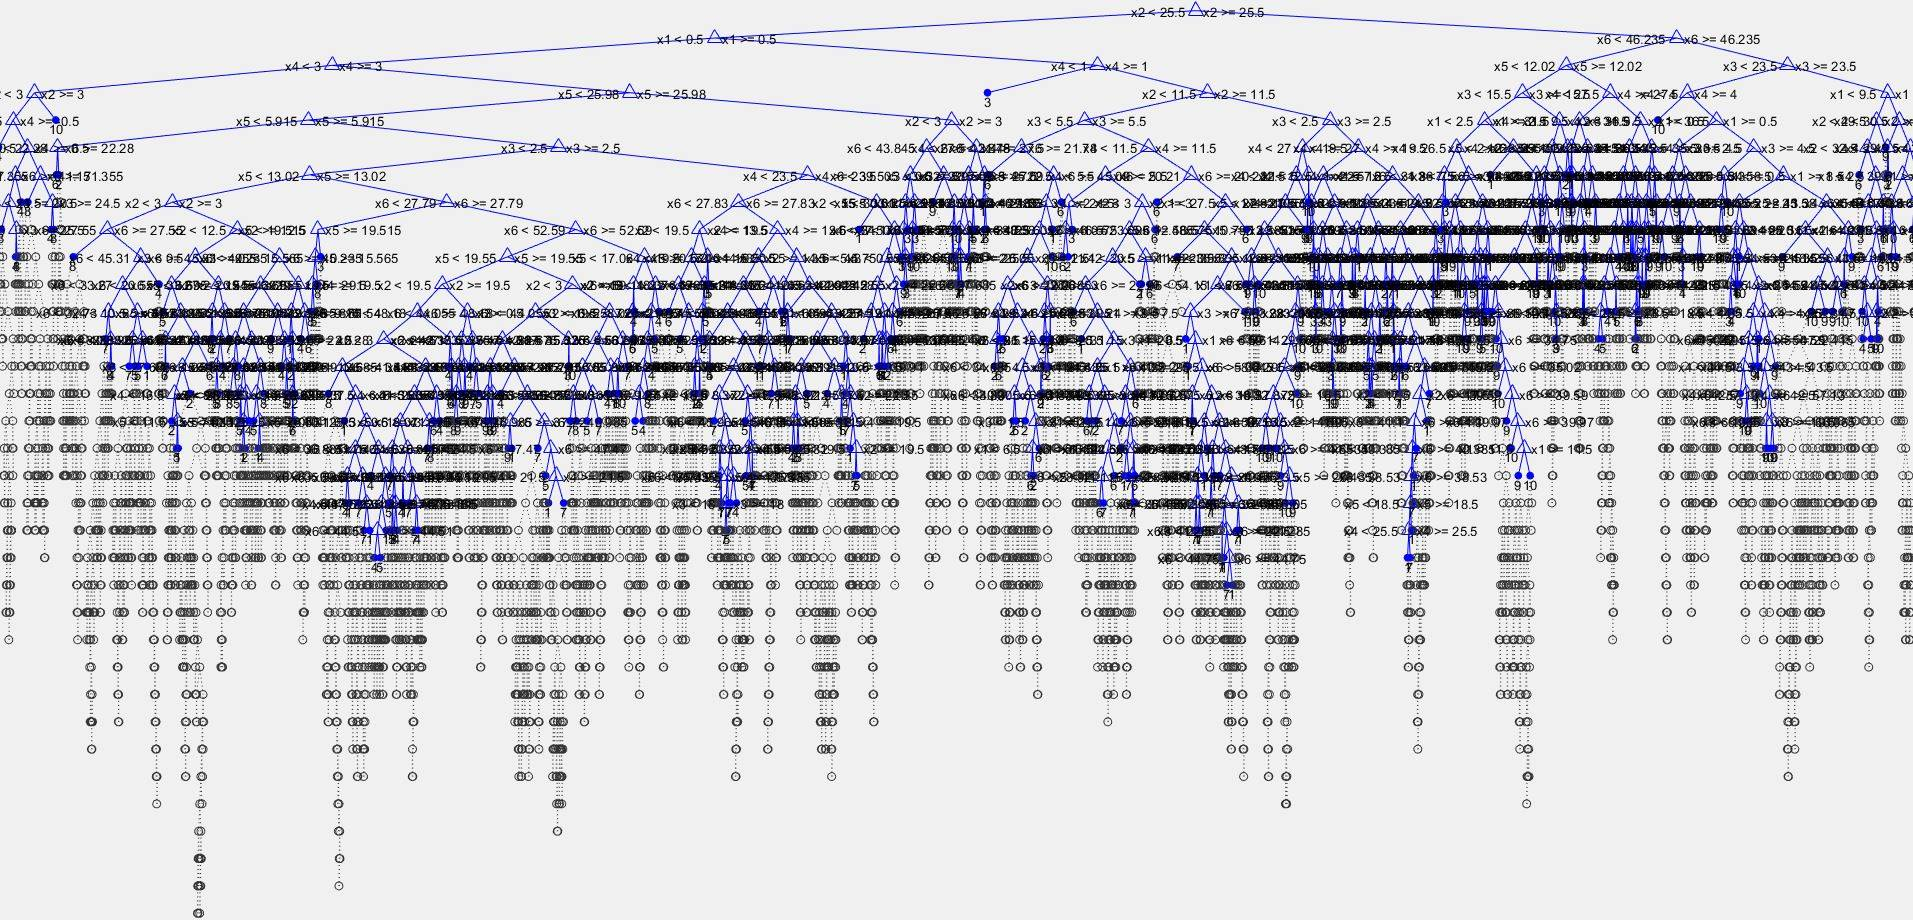
\includegraphics[width=0.95\textwidth]{04-tree}
	\caption{Árbol resultante después de la poda}
	\label{fig:tree}
\end{figure}

En la tabla~\ref{tab:tree} se pueden observar los resultados obtenidos.

\begin{table}[htbp]
\centering
\caption{Resultados de los experimentos con Árboles de Decisión}
\label{tab:tree}
\begin{tabular}{@{}cccc@{}}
\toprule
Train & Test  & Nivel de Poda & Precisión (\%) \\ \midrule
5109  & 25545 & 0 & 50.91   \\
5109  & 25545 &  13 & 51.70   \\
25545 & 5109  & 0 & 55.65   \\
25545 & 5109  & 65 & 56.86   \\ \bottomrule
\end{tabular}
\end{table}

Como se puede apreciar en la Tabla~\ref{tab:tree}, no hubo una gran diferencia entre el peor y el mejor desempeño a pesar de que la cantidad de datos de entrenamiento fue cinco veces mayor.
Además, la precisión sólo aumentó 1.2\% después de realizar la poda.
Se esperaba que la precisión fuera un poco menor después de realizar la poda ya que se están eliminando ramas para disminuir el tamaño del árbol y generalizar.
Sin embargo, la generalización de esas ramas provocó un incremento en la precisión, lo cual pudo haber sido por eliminar un poco el sobreajuste que se generó durante el entrenamiento.

El código fuente del árbol de decisión está en la carpeta de la tarea, con el nombre \texttt{04-decisiontree.m}, y fue hecho en \texttt{MATLAB}.

\subsection{Support Vector Machine}
\label{subsec:svm}

Para la implementación del Support Vector Machine se utilizó la librería \texttt{LIBSVM}, la cual está disponible como código abierto en la página de la Universidad de Taiwan de Ciencia y Tecnología~\cite{LIBSVM}.

Tras leer la documentación, se generó un \textit{script} para entrenar el SVM con los siguientes parámetros:

$$\mathtt{-s 0 -t 2 -g 0.00048828125 -c 8192 -m 300}$$

donde:

\begin{itemize}
	\item \texttt{-s 0}: tipo de SVM, SVM de clasificación.
	\item \texttt{-t 2}: kernel 2, RBF (Gaussiano): $e^{(-\gamma |u-v|^2)}$
	\item \texttt{-g 0.00048828125}: valor de $\gamma$.
	\item \texttt{-c 8192}: valor de $C$, penalización por datos mal clasificados por el SVM.
	\item \texttt{-m 300}: memoria disponible para el script, en este caso se asignó un buffer de 300 MB.
\end{itemize}

Cabe mencionar que los valores de $\gamma$ y $C$ fueron encontrados usando optimización local y validación cruzada con las mismas herramientas de la librería.

Con estos parámetros, y usando el conjunto de entrenamiento por defecto (1000 instancias de entrenamiento y 5000 de prueba) se logró clasificar correctamente el 56\% de los datos.
Usando los datasets de manera inversa (5000 para entrenamiento y 1000 para prueba) se alcanzó una precisión de poco más del 60\%.
Los detalles adicionales de precisión se encuentran en la Tabla~\ref{tab:svm}.

% Please add the following required packages to your document preamble:
% \usepackage{booktabs}
\begin{table}[htbp]
\centering
\caption{Resultados de los experimentos con SVM}
\label{tab:svm}
\begin{tabular}{@{}cccc@{}}
\toprule
Parámetros & Train & Test  & Precisión (\%) \\ \midrule
Default    & 5109  & 25545 & 47.4731   \\
Opt. Local & 5109  & 25545 & 56.6647   \\
Default    & 25545 & 5109  & 57.4476   \\
Opt. Local & 25545 & 5109  & 60.8925   \\ \bottomrule
\end{tabular}
\end{table}

Como se aprecia en la Tabla~\ref{tab:svm}, la aplicación de optimización local para la selección de los parámetros incrementa la precisión de la predicción.
Sin embargo, el mayor incremento (casi 10\%) aparece cuando se utilizan más datos para entrenamiento.
La combinación de optimización local y un aumento considerable en el tamaño del set de entrenamiento permite obtener cerca del 60\% de precisión.
Esto refuerza la noción de que el margen de precisión de los SVM disminuye a medida que el tamaño del conjunto de entrenamiento incrementa.
Un comportamiento `opuesto' ocurre en otros modelos como \textit{Naive Bayes},
donde el modelo se comporta mejor con pocos datos de entrenamiento.
Un SVM muestra mejor desempeño asintótico, sin embargo, si existen más ejemplos para entrenar.

El código fuente del SVM está en la carpeta de la tarea con el nombre \texttt{04-svm.m}, y fue hecho en \texttt{Octave}.

\section{Conclusiones y Reflexiones}
\label{sec:conc}

Este reporte incursionó en la implementación de dos clasificadores muy conocidos de \textit{Machine Learning},
los árboles de decisión y las máquinas de vectores de soporte.
Cada uno tiene ventajas y desventajas, y la precisión obtenida por ambos modelos está dentro del mismo rango.
Es importante recalcar que el \textit{dataset}, a pesar de ser muy grande no da una idea muy clara para ambos métodos de clasificación.
Es posible que el hecho de que sea multiclase (10 clases) y el reducido número de atributos (7 en total) haga que el aprendizaje sea más complicado.
El ejercicio estuvo muy interesante, pues reforzó la idea de que los métodos de clasificación necesitan de muchos datos para tener un buen desempeño.
Además, se utilizaron módulos y \textit{toolboxes} de la literatura que permiten ver las dificultades de la implementación de los clasificadores.

\bibliographystyle{splncs03}
\bibliography{04-biblio}

\end{document}